\section{Description of OpenVAS Setup} \label{sec:setup}

OpenVAS Is a framework that offers services and tools that provide a complete and powerful solution for vulnerability scanning and vulnerability management as well as it allow us to identify different security risks in a system (not only scan ports). So the main aim of OpenVAS is to assert a system (vulnerability identification). At the same time it allows us to make several types of reports on detected vulnerabilities and to propose associated solutions. In relation with the architecture, OpenVAS consists in the client part (OpenVAS CLI command line/Greenbone assistant) that interacts with two services called OpenVAS scanner (core) and OpenVAS management (back-end part). The first one performs tasks related with classification/filtering of the scanned results, database control and user administration. On the other hand the OpenVAS scanner executes the NVT (Network Vulnerability Test) conformed by routines that check known vulnerabilities into the system.

In figure 1, the network setup is described as clients connecting to the OpenVAS server ($theoden.ce.chalmers.se$ and in our case in a remote way SSH) via the client Greenbone that manages the  requests and send them to the OpenVAS Manager in order to scan the hosts. In this case the network contains 3 hosts (this report is based on scans of $rome.secnet$).

Scanning methods allow to detection and handling of known security problems, can help identify rogue machines on the network and provide useful information about the 	devices that can be useful in security management and tracking.
There are different types of vulnerability scanning such as network-based that scans a 	number of hosts on the network (port scanners, web application scanners) and host-	based scanners where the same host is scanned.

The scanning results tell us the results of the prioritised vulnerabilities (high, 	medium, low) according to the impact on the system and the total amount for each category. In our case we made a scan against the target host $rome.secnet$ and no 	vulnerabilities have been found. Once the scan has finished one vulnerability 	assessment report is available giving us useful information. It contains the results of the executed plugins associated with the corresponding subnet, host, port and severity.

To perform as scan using OpenVAS, a new target has to be created by clicking on Configuration/add a new 	target. Once there, some fields have to be filled (Name, host IP, port list). After, is it necessary to generate a new task clicking on scan management/new task for the execution of the analysis and evaluation. Finally the task must be executed and a report with the results is generated.

%\inlinetodo{Why you choose the different NVTs and the chosen configurations?}

Depending on your needs and your budget there are a number of different well known vulnerability scanners available. Furthermore, multiple options are available depending on the type of system to be tested. For example scanning all ports in many cases takes too long. Many ports are normally not being used. For most scans it is often enough to scan the ports registered with the IANA.

\begin{figure}[htb]
  \centering
  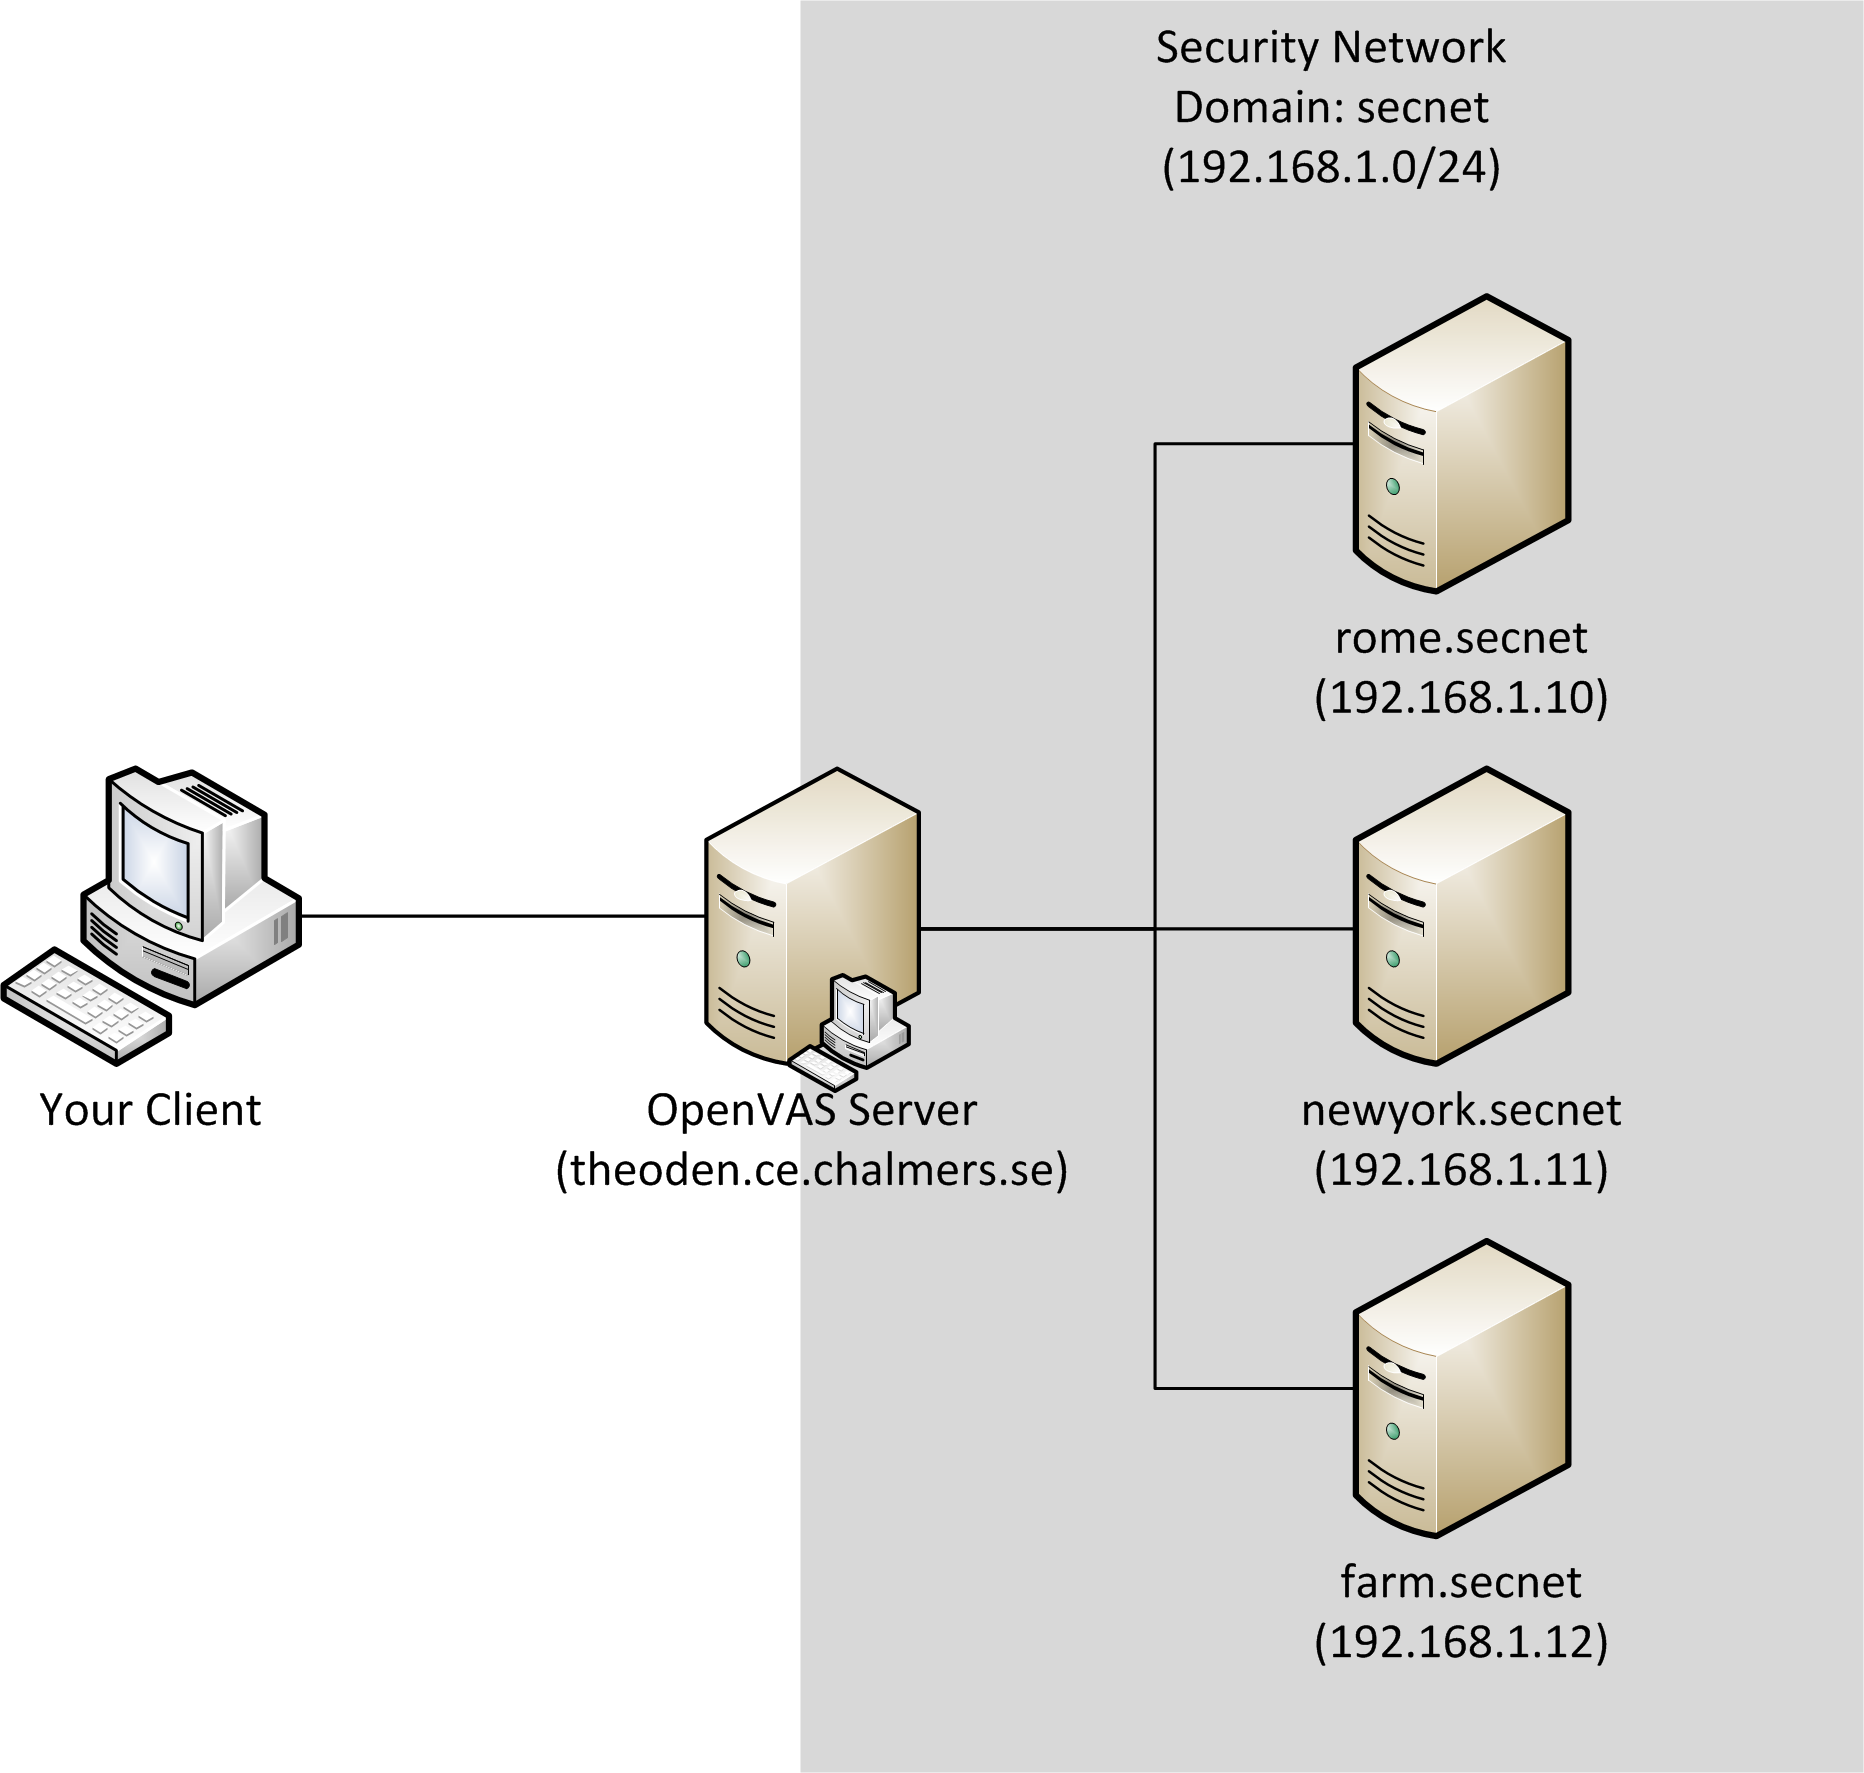
\includegraphics[scale=.4]{figures/setup.png}
  \caption{The laboratory network setup} \label{fig:setup}
\end{figure}



%\subsection{Port Scanning}

%\inlinetodo{text, figures, and tables if needed. Figure captions are below of figures, and Table caption should be above them.}


%\subsection{Fingerprinting}

%\inlinetodo{text, figures, and tables if needed}


%\subsubsection{Service Fingerprinting}
%\inlinetodo{text, figures, and tables if needed}

%\subsubsection{Remote Host Fingerprinting}
%\inlinetodo{text, figures, and tables if needed}


%\subsection{Vulnerability Scanning}

%\inlinetodo{text, figures, and tables if needed}
